%Type of document
\documentclass[a4paper, 12pt]{report}

%For easy management of document margins and the document page size
\usepackage[right=3.5cm,left=3.5cm,top=3.5cm,bottom=3.5cm]{geometry}

%Allows to insert graphic files within a document
\usepackage{graphicx}

%Sup­ports com­pressed, sorted lists of nu­mer­i­cal ci­ta­tions, and also deals with var­i­ous punc­tu­a­tion and %other is­sues of rep­re­sen­ta­tion, in­clud­ing com­pre­hen­sive man­age­ment of break points
\usepackage{cite}

%It gives LaTeX the possibility to manage links within the document or to any URL when you compile in PDF
\usepackage{hyperref}

%To choose the font encoding of the output text
\usepackage[T1]{fontenc}

%To choose the encoding of the input text
%Consente di usare le lettere accentate
\usepackage[latin1]{inputenc}

%It provides the internationalization of LaTeX. It has to be loaded in any document, and you have to give %as an option the main language you are going to use in the document
\usepackage[english]{babel}

%Allows to write algorithms
\usepackage{algorithm}
\usepackage{algpseudocode}

\normalfont
%Forza LaTeX ad una spaziatura uniforme, invece di lasciare più spazio
%alla fine dei punti fermi come da convenzione inglese
\frenchspacing
%Modifica della spaziatura interlineare
\linespread{1.3}

%Inizia il documento
\begin{document}

%Creazione di un frontespizio personalizzato
\begin{titlepage}

\begin{center}
\Large
\textbf{POLITECNICO DI MILANO} \\
\Large
School of Industrial and Information Engineering \\
Computer Science and Engineering
\end{center}

\addvspace{0.8cm}
%PER INSERIRE IMMAGINE
\begin{figure}[h]
\begin{center}

\includegraphics[width=7cm]{cpt/img/polimi.png}
\end{center}
\end{figure}

\addvspace{0.1cm}
\begin{center}
\LARGE

\textbf{Design and Implementation of Mobile Application Project: Safe Car \\
Design Document}

\end{center}

\addvspace{0.5cm}
\Large
\begin{center}
\begin{tabular}{p{1\textwidth}p{0.3\textwidth}}
Course Professor: Prof. Luciano BARESI \\
\end{tabular}
\end{center}

\addvspace{0.6cm}
\Large
\begin{center}
\begin{tabular}{p{0.6\textwidth}p{0.6\textwidth}}
& Authors: \\
& Mattia	CRIPPA		1039725\\
& Alberto PIROVANO	10396610
\end{tabular}
\end{center}

\vfill
\Large
\begin{center}
Academic Year 2017--2018
\end{center}
\end{titlepage}

\clearpage

\begin{abstract}
SafeCar is an application that has been designed to help the driver in improving its driving style. 
On one side it offers the possibility to inspect the historical user data, and on the other side it provides a hint generation engine during the trip .
The core algorithm of the application communicates in an asynchronous way with a physical object that has to be plugged into the car. This object is the interface between the car and the application, and once connected with it the application is able to access and process the data about the navigation.
During the trip the application analyses these data, processing them to profile the driving style. In addition it generates an index representing a summary of a specific moment of the trip. Based on this index, another algorithm generates a hint message.
This procedure is performed in loop, so the application generates hints continuously during the trip and through these hints the user can obtain some indications about how to improve his driving style.
\end{abstract}

\tableofcontents
\clearpage

\listoffigures
\clearpage

\chapter{Introduction} \label{chap1}
The \textit{Design Document} is a document meant to provide documentation which will be used to help developers in implementing the entire system by providing a general description of the architecture and the design of the system to be built.

\section{Purpose}
The purpose of the Design Document is to provide a description of the system detailed enough to understand which are the components of the system, how they interact, which is their architecture and how they will be deployed. The level of the description is high enough for all the stakeholders to capture the information they need in order to decide whether the system meets their requirements or in order to begin the development work.

\section{Scope}
This document provides a detailed description of \textit{Safe Car} software design and architectural choices. Every portion of the document is designed itself to be comprehensible, but a big picture of the system must be present to the reader in order to obtain the best knowledge on the matter when consulting this document.

\section{Definitions \& Acronysms}
We are going to use a set of specific terms, each one referring to a specific abstract or physical object:

\begin{enumerate}
	\item \underline{Plug}: It is a smart object that the user has to buy and that has to be plugged inside the h732 port of the car. It has to have Bluetooth functionalities enabled
	\item \underline{Trip}: An abstract concept data structure containing all the information about a travel
	\item \underline{Badge}: An abstract object that refers to a specific unlocking condition. It can be locked or unlocked
\end{enumerate}
In the document are often used some technical terms whose definitions are here reported:

\begin{enumerate}
	\item \underline{Layer}: A software level in a software system
	\item \underline{Tier}: An hardware level in a software system
\end{enumerate}
We also need some application specific terminology:

\begin{enumerate}
	\item \underline{DSI}: Driver Safety Index
	\item \underline{ALG1}: High-level hint generation algorithm
	\item \underline{ALG2}: DSI computation engine
	\item \underline{ALG3}: Low-level hint generator agent
\end{enumerate}

\section{Document Structure}
This document is intended for individuals directly involved in the development of Safe Car application. This includes software developers, project consultants, and team managers. This document is not meant to be read sequentially; users are encouraged to jump to any section they find relevant. Below is a brief overview of each part of the document:

\begin{enumerate}
	\item \textbf{Introduction:} This section gives general information about the Design Document of Safe Car application
	\item \textbf{System Overview:} This section contains an overview of the application and its primary functionalities. It also contains assumptions and constraints followed during the design of the software
	\item \textbf{Architectural Design:} This section exposes in details the design chosen for the architecture of the system to be
	\item \textbf{User Interface Design:} This section provides the detailed design information for each component in the current delivery
\end{enumerate}
\clearpage

\chapter{System Overview} \label{chap2}
The aim of our project is to develop an android application which can be used in the real world.\\
In order to use this application, the driver has to register as a user of the service. The \textit{Registration and Login} procedures can be performed via the custom application functionality or via Google Plus APIs.
The user can change his password, drop the account and modify data related with his profile whenever he wants.
At this point the application flow develops in two different ways:

\begin{itemize}
	\item If the user's smartphone is not in the radio scan area of the Plug, he can only inspect user related data about his history usage with the application. He can consult the performed trips, his profile data or the gained badges
	\item On the other side, if the user's smartphone is close to the Plug, he can pair his device with that Plug and, after the procedure has succeeded, he can start a new trip. Now the \textit{Driving Experience} actually begins. After this moment, the application will follow the user in his driving experience by asking to the plug data about the navigation, for example the acceleration rate or the frequency with which the user is breaking. On the base of these data, the driver will be provided with several hints about how to improve her driving style, until he decides to end the trip
\end{itemize}
When the trip finishes, the application will provide an after trip report graphical showing the followed route on a custom map.\\	
The application is comprised of two main features:

\begin{enumerate}
	\item \textbf{After Trip data presentation:} The user can inspect inspect the details of the just finished trip once the trip has finished. In this screen the user can see:
	\begin{itemize}
		\item The route he followed, shown in a custom google maps widget
		\item A general report about the just finished trip providing the departure, the arrival, the date of the trip, the kilometres traveled, the time that the trip took and the Driver Safety Index (DSI), that estimates the quality of the drive
	\end{itemize}
	\item \textbf{During Trip functionalities:} This functionality, instead, is provided by the core Safecar?s algorithm. This algorithm is an engine that has the role of estimating the Driver Safety Index by using navigation data coming from the car. This device is a smart object, a plug, that has to be inserted in the custom car gate and that has the capability of sending cleaned and custom driving style data to the connected device
\end{enumerate}
Using all these data the algorithm computes the \textit{Driver Safety Index} (DSI). The engine architecture is easily exchangeable, given that the application is built in a parametric way. Building a more complex algorithm is only a matter of replacing the specific piece of code (a method) with another one that takes as input the same data and generates a same type index, but by implementing a different, maybe more complex, logic.
In order to provide the user with an almost continuous feedback about his driving style, this engine recomputes the DSI index once every 30 seconds.
Its computation is done in a dedicated separate thread that generates the current piece of advice to be sent to the user by simply switching on the value of the DSI. This hint is conveyed by filling a specific screen on the application.

\clearpage
\section{System constraints:}
These are the constraints which must be met in order to allow the application to work correctly:

\begin{itemize}
	\item User of the mobile should have partial internet access:
	\begin{itemize}
		\item The user application has to have the internet access at least during the login and the logout procedure. In fact, during the actual use of the application it doesn?t need the data connection
	\end{itemize}
	\item User's device should support bluetooth:
	\begin{itemize}
		\item The application needs the bluetooth for the interactive part, the one in which the app follows the user during the navigation. During the offline part, it doesn?t need any bluetooth capability
	\end{itemize}
	\item User's device should support geolocalization:
	\begin{itemize}
		\item The application needs the geolocalization for the interactive part, the one in which the app follows the user during the navigation. During the offline part, it doesn?t need any geolocalization capability
	\end{itemize}
\end{itemize}
\clearpage

\chapter{Architectural Design} \label{chap3}
This section exposes Safecar Architectural Design in a complete e comprehensible way.

\section{Layers}
The software architecture that has been chosen follows the principles of the \textit{Model-View-Controller} architectural pattern. Therefore three main software components have been identified and those are without any coup de theatre: the Model, the View and the Controller.

\subsection{View}
The role of this Layer is the one of processing Clients commands, and of converting them into requests addressed to the Controller layer.

\subsection{Controller}
In this second Layer are included all the software components that implement the system logic, the authentication logic and the high level data primitives. The application logic is handled by the Firebase cloud authentication services and by some ad hoc authentication components.

\subsection{Model}
The third and last Layer is the Model, that should guarantee a high level interface to store and manage all the Safecar relevant data. It is provided by Firebase cloud database.

\section{Tiers}
The system can be divided in two different Tiers, which are the Clients and the Cloud Database

\begin{enumerate}
	\item \textbf{Clients}: This is the android mobile application. The view and the controller layers are mapped on this Tier. A thin model is also present on the Client Tier
	\item \textbf{Cloud Database}: In this Tier it is hosted the Database that allows the service data persistence. The Model layer is entirely mapped to this Tier
\end{enumerate}
This architecture, with three different Layers and two different Tiers, makes possible to have a Client-Server style with a Fat-Client and a Thin-Server. This is due to the mapping of the View, the Controller and the thin model to the Client and the complete Model to the Server.

\section{Cloud and Local Model}
Once the user logs in, the application downloads all the user related data from the cloud model and dumps them into a local copy called \textit{Local Model}. \\
This wrapper is build through the Realm real time database APIs. In particular, when the user modifies some piece of data, the application updates its local model item, leaving the cloud model unchanged.\\
For example, this happens when the user decides to drop a trip, to add a trip, to drop a plug or to add a new plug. 
For this, there is no need of internet connection after the login and before the logout procedures, in fact all the modifications are performed locally.\\
When instead the user decides to log out, the application understands which are the data items that have been modified and uploads their modifications to the cloud model in order to make it consistent with the local one. 
After pushing the modifications the controller drops the local model and exits the user session.

\section{Application components and their interaction}
In the following section are deeply covered all the architectural aspects that characterize the software to be. In particular, here it is explained which are all the components of this application and how they interact in order to have a complete functional software.

\subsection{Login component}
This component handles the user's login procedures and it provides either the \textit{Google+} authentication service or the email and password authentication service.

\subsection{Sign in component}
It manages the Sign in procedures, that is the generation of a new user object.

\subsection{Reset password component}
It is in charge of handling the procedure of change password for the user that has been registered through the email and password login procedure.

\subsection{Logout component}
It has the responsibility of maintaining the consistency between the Cloud Model and the Local Model.

\subsection{Personal data component}
This is responsible of computing and handling the modifications to the profile information.

\subsection{DSI computation engine}
This is the most important component, in fact is in charge of:

\begin{itemize}
	\item Ordering and placing the trips contained in the local model into in the four dedicated tabs. This is done by using four software components, respectively \textit{DateComparator}, \textit{DSIComparator}, \textit{KMComparator} and \textit{DurationComparator}
	\item Handling the sampling of position pins during the trip. It also stores them into the current trip object. This is done by the \textit{TripHandler} thread, an asynchronous task. It is spawned when the trip starts and it autonomously handles it
	\item Through a call to the first algorithm, namely \textit{ALG1}, it computes the DSI index through the \textit{DSIevaluator} asynchronous task
	\item After that, Safecar exploit the feature of the second algorithm, namely \textit{ALG2} to compute the current hint
\end{itemize}

\subsection{Plug component}
This component implements the logic for pairing, managing and using the abstract interface of physical plugs.

\subsection{Badges component}
This components implements the procedure that, by using the user's data, computes the badges that the user currently holds.

\section{External services}
Safecar is fully integrated with several external services

\subsection{Firebase database}
Safecar makes use of the great Firebase cloud database to store the data about trips, users and plugs. It represents the persistent storage of the application.

\subsection{Firebase authentication}
Firebase is also great for the authentication capabilities that it offers. Safecar exploits the Google authentication services but is straightforward to integrate also Facebook, Twitter and GitHub.

\subsection{Bluetooth core service}
In order to pair the user's device with the selected plug, Safecar uses the core \textit{Bluetooth Adapter} to interface with the physical device plugged in the car.

\subsection{Geolocalization core service}
During the trip, Safecar periodically samples location data in order to be able to precisely track the trip's route.

\subsection{Realm real-time database}
In order to ensure consistency , Safecar uses two databases services, one being a cloud one and the other one being a local and real-time one. Realm is used to ensure database queries to be fast, efficient and precise.

\subsection{Gilde image loader}
In order to have the feature of loading profile images from disk, the application uses a third-party set of APIs, Gilde.

\subsection{Picasso image cropper}
To provide fancy cropping features to the profile images, Safecar exploits the power of another third-party set of APIs, Picasso.

\section{Algorithms}
The application wraps the customizable algorithms into pluggable blocks. It is then possible to change those blocks with different and maybe more complex algorithms.\\
The important fact is that the new algorithm will respect the following interface:

\begin{itemize}
	\item \textbf{ALG1}: It takes as an input the \textit{MAC} address of the current plug and returns the current DSI. Now we can face two cases:
	\begin{itemize}
		\item The application is run on a device paired with a real plug. In this case \textit{ALG1} has to:
		\begin{enumerate}
			\item Register itself to the plug
			\item Connect with the plug
			\item Periodically ask the plug for some kind of data
			\item Clean and parse the data and put them into a custom data structure
			\item Pass the parsed data structure to \textit{ALG2}
			\item Get the DSI from \textit{ALG2}
			\item Pass the DSI to \textit{ALG3}
		\end{enumerate}
		\item The application is run on a device that has no access to a real plug. In this case \textit{ALG1} has to:
		\begin{enumerate}
			\item Stash the current input
			\item Call \textit{ALG2}
			\item Get the DSI from \textit{ALG2}
			\item Pass the DSI to \textit{ALG3}
		\end{enumerate}
	\end{itemize}
	\item \textbf{ALG2}: It takes as an input the parsed data from \textit{ALG1} and returns a DSI. It can be of two types:
	\begin{enumerate}
		\item Memory based:
		\begin{itemize}
			\item It computes the current DSI from the current input
			\item It has to store all the previous DSI scores into a data structure and has to generate the current DSI by combining them in some way. An example can be to construct a discounted weighted average of the DSI over time to generate a value of the DSI that could be related to the current sample but also not blind with respect to the past driving style
		\end{itemize}
		\item Blind:
		\begin{itemize}
			\item It computes the current DSI only from the current data structure in input
		\end{itemize}
	\end{enumerate}
	\item \textbf{ALG3}: It is an agent that takes as input the computed DSI and returns an hint string. It can be viewed as an agent that takes as input a percept and returns a decision. It can be:
	\begin{enumerate}
		\item \underline{Simple reflex}: It matches the percept on a rule set and returns the decision related to the matched rule
		\item \underline{Model based reflex}: It stored the percept sequence and, through a model, matches a rule
		\item \underline{Goal based}: Basing on the current percept, on the model and on a goal specification, it returns the best hint to reach the goal. In this case the DSI computation can be jumped and this algorithm can work on the factored representation returned by \textit{ALG1}. This algorithm is a tree search or a graph search.
	\end{enumerate}
\end{itemize}

\clearpage

\chapter{User Interface Design} \label{chap4}
Here are presented some mockups that represent an idea of the structure of the application pages.

\clearpage
\section{Splash Screen and Registration \& Login Pages}
These mockups show an idea of the \textit{Splash Screen} and \textit{Registration \& Login} pages of the application. The Registration and Login Page allow the user of the application to register as a user of the service and this can be performed via the custom application functionality or via external providers.\\

\begin{figure}[htbp]
  \centering
  \begin{minipage}[b]{0.45\textwidth}
    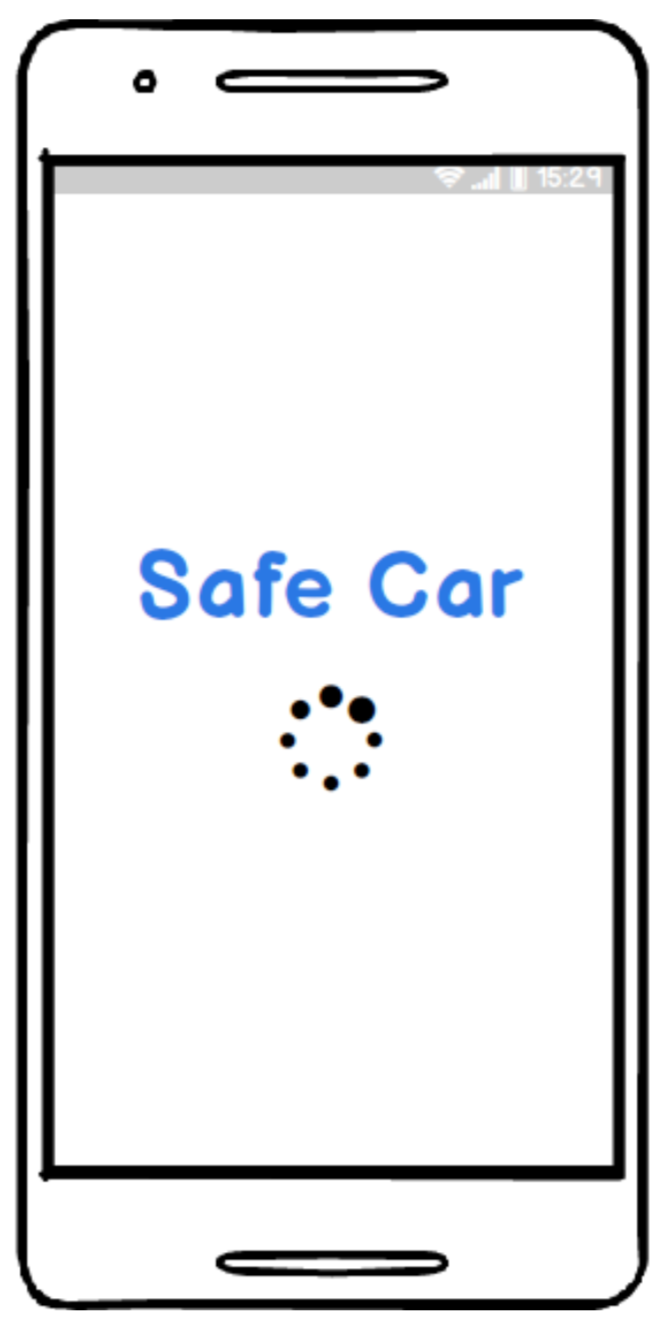
\includegraphics[width=\textwidth]{cpt/img/SplashScreen.png}
    \caption{Splash Screen}
  \end{minipage}
  \hfill
  \begin{minipage}[b]{0.45\textwidth}
    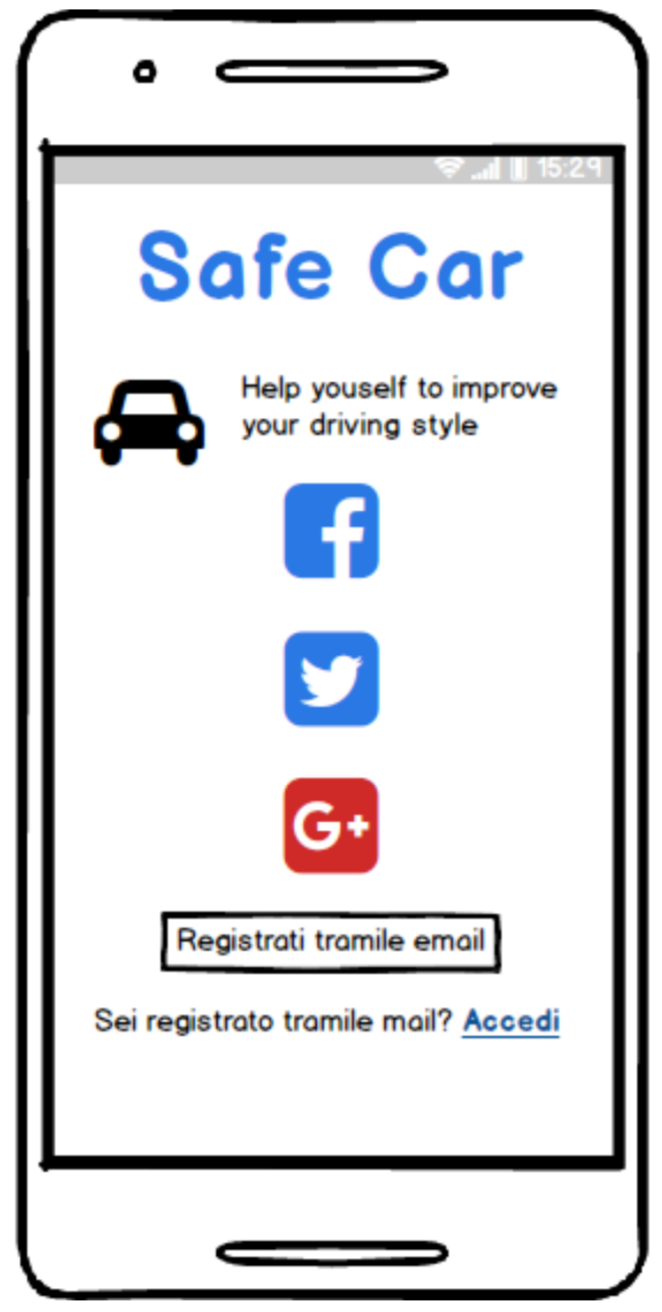
\includegraphics[width=\textwidth]{cpt/img/Login.png}
    \caption{Registration \& Login}
  \end{minipage}
\end{figure}

\clearpage
\section{Home Page}
These mockups show an idea of the \textit{Home Page} of the application. The Home Page presents a \textit{TabView} through which the user can navigate in order to inspect his history trips and a \textit{Navigation Drawer Menu} through which the user can reach other pages of the application.\\

\begin{figure}[htbp]
\centering
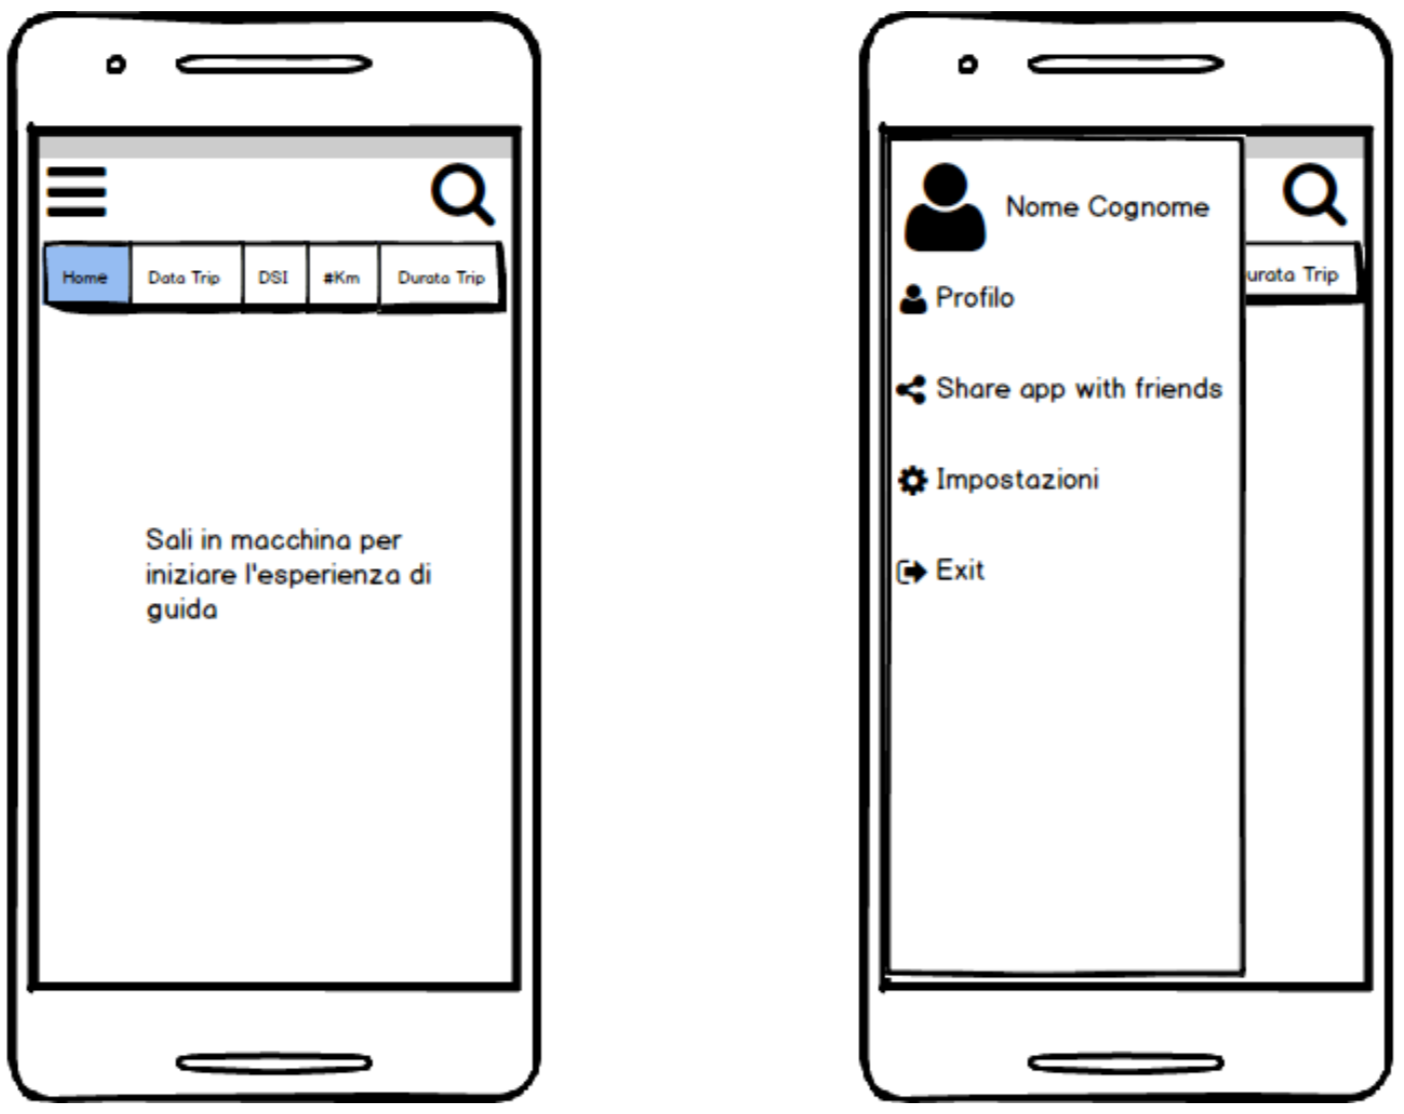
\includegraphics[width=\textwidth]{cpt/img/HomePage.png}
\caption{Home Page}
\end{figure}

\clearpage
\section{During Trip Page}
These mockups show an idea of the \textit{During Trip Page} of the application. The During Trip Page presents a \textit{View} where \textit{Hints} produced by the application are loaded and viewable by the user. The user can interact with the application using two buttons: the first one is a \textit{Pause/Resume} button which allow the user to pause the trip, without stopping it, if he wants to take a break from the driving session and, then, resume it; the second one, instead, is a \textit{Stop} button which allow the user to end the driving experience.\\

\begin{figure}[htbp]
\centering
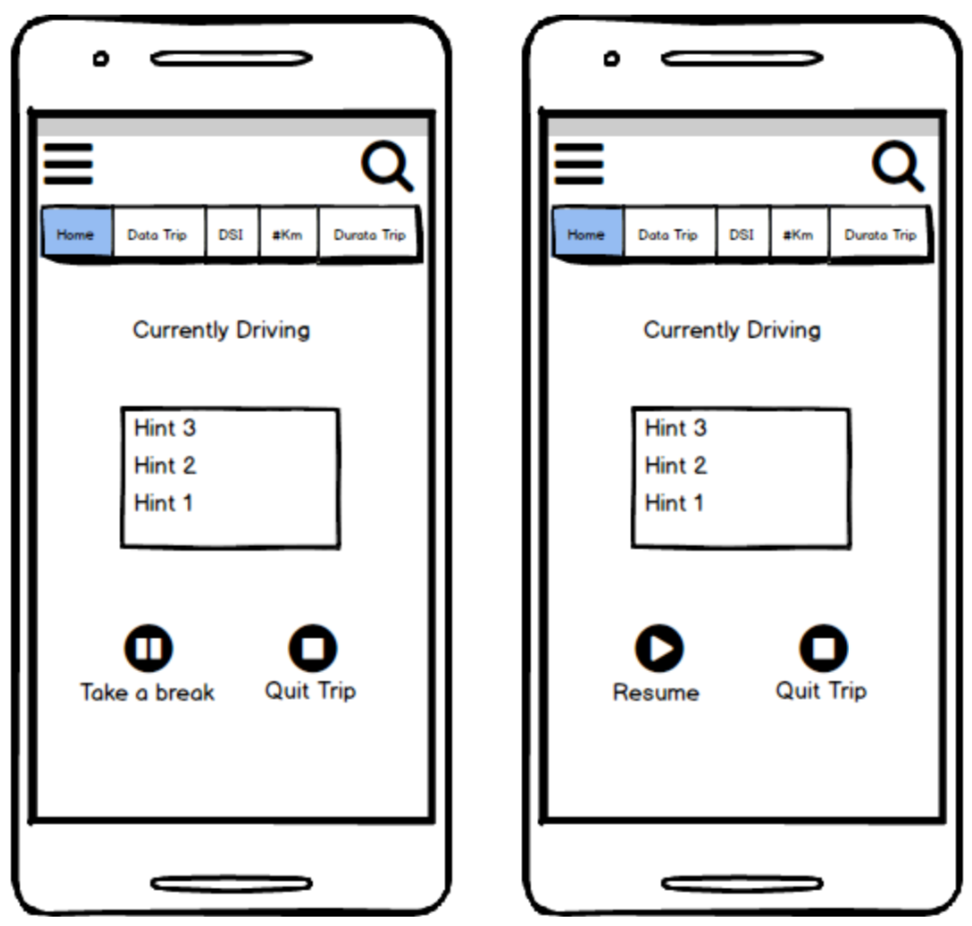
\includegraphics[width=\textwidth]{cpt/img/DuringTrip.png}
\caption{During Trip}
\end{figure}

\clearpage
\section{Report Page}
This mockup show an idea of the \textit{Report Page} of the application. The Report Page is showed when the user inspect one of his history trips or when he complete a driving session pushing the \textit{Stop} button. This page allow the user to see all the details about his trip including data like: the trip's date, duration and length, the DSI score and the path he made.\\

\begin{figure}[htbp]
\centering
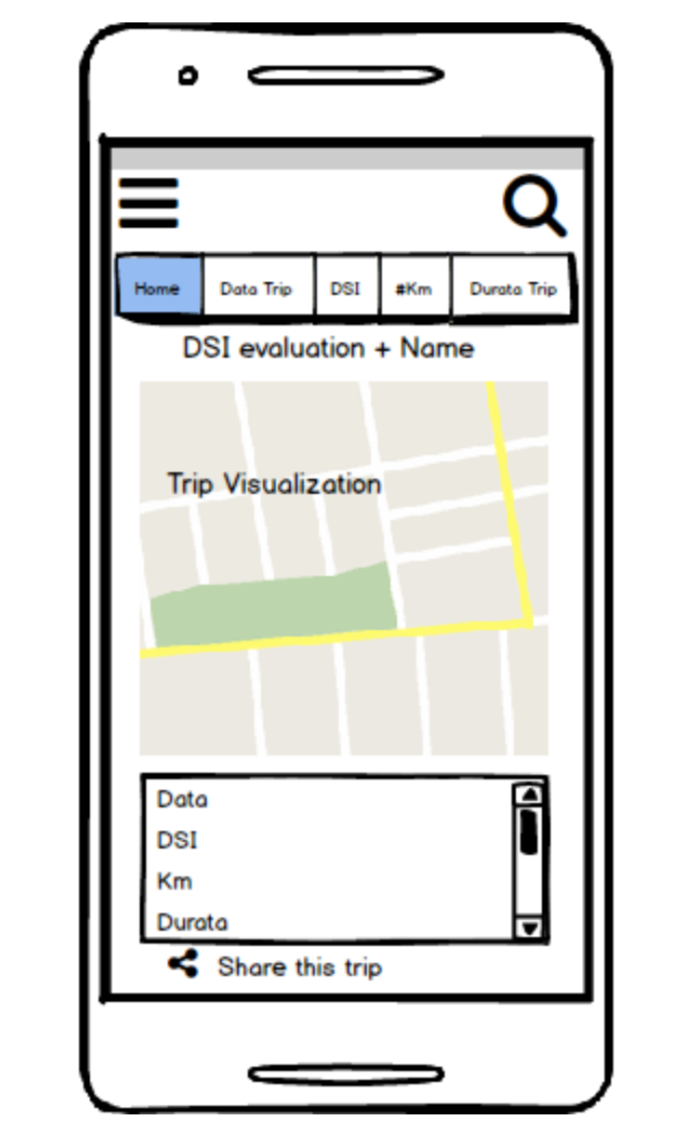
\includegraphics[width=0.7\textwidth]{cpt/img/ReportPage.png}
\caption{Report Page}
\end{figure}

\clearpage
\section{Profile Page}
These mockups show an idea of the \textit{Profile Page} of the application. The Profile Page shows information about the user like his name, surname, email address, driver level and also some badges that he can unlock meeting specific conditions. Each badge is clickable and let the user know about its locked/unlocked status.\\

\begin{figure}[htbp]
\centering
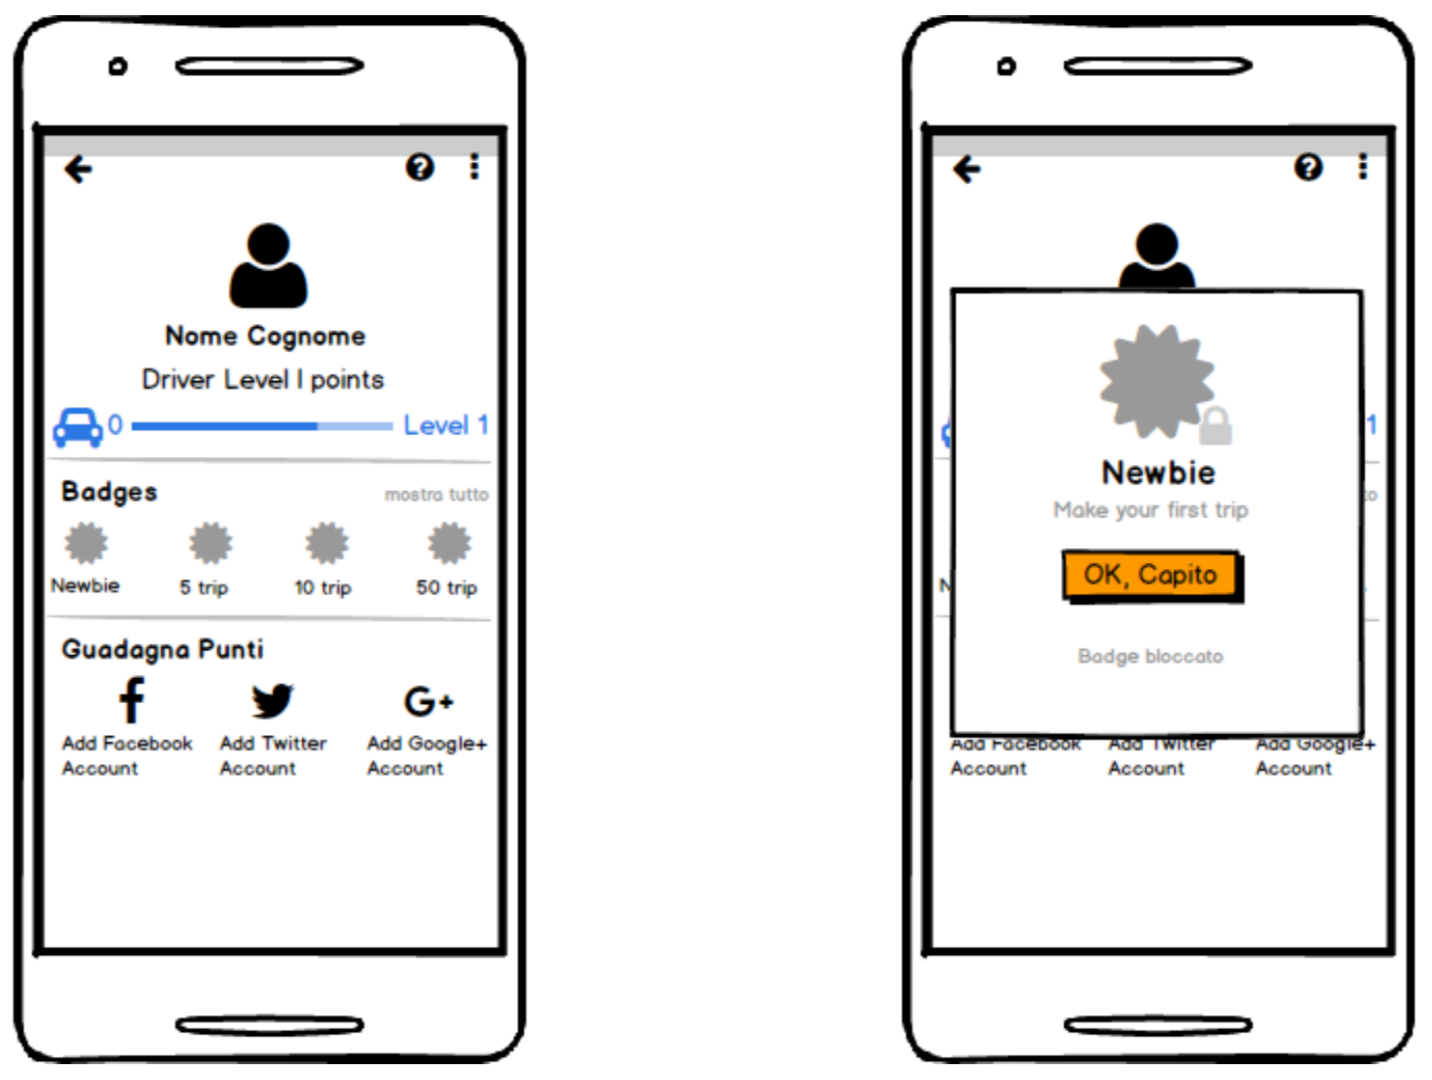
\includegraphics[width=\textwidth]{cpt/img/ProfilePage.png}
\caption{Profile Page}
\end{figure}

\clearpage
\section{Settings Page}
This mockup show an idea of the \textit{Settings Page} of the application. The Settings Page allow the user to manage some settings of the application like push notifications and smart objects. This page also allow the user to see some info about the application and send feedback in order to improve it.\\

\begin{figure}[htbp]
\centering
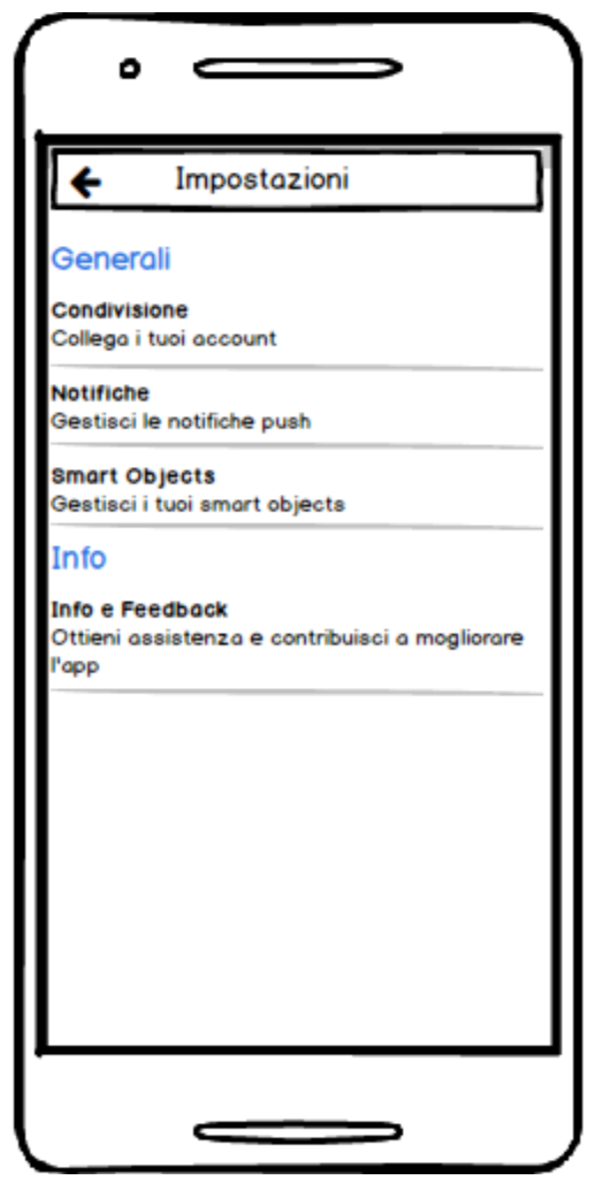
\includegraphics[width=0.55\textwidth]{cpt/img/SettingsPage.png}
\caption{Settings Page}
\end{figure}

\clearpage
\section{Smart Objects Page}
These mockups show an idea of the \textit{Smart Objects Pages} of the application. The Smart Objects Pages allow the user to manage smart objects which are necessary for the application. Using a bluetooth scanner the user can pair his device with a plug used to retrieve relevant information about the current driving session and he can also manage all the paired plugs, inspecting or deleting them.\\

\begin{figure}[htbp]
\centering
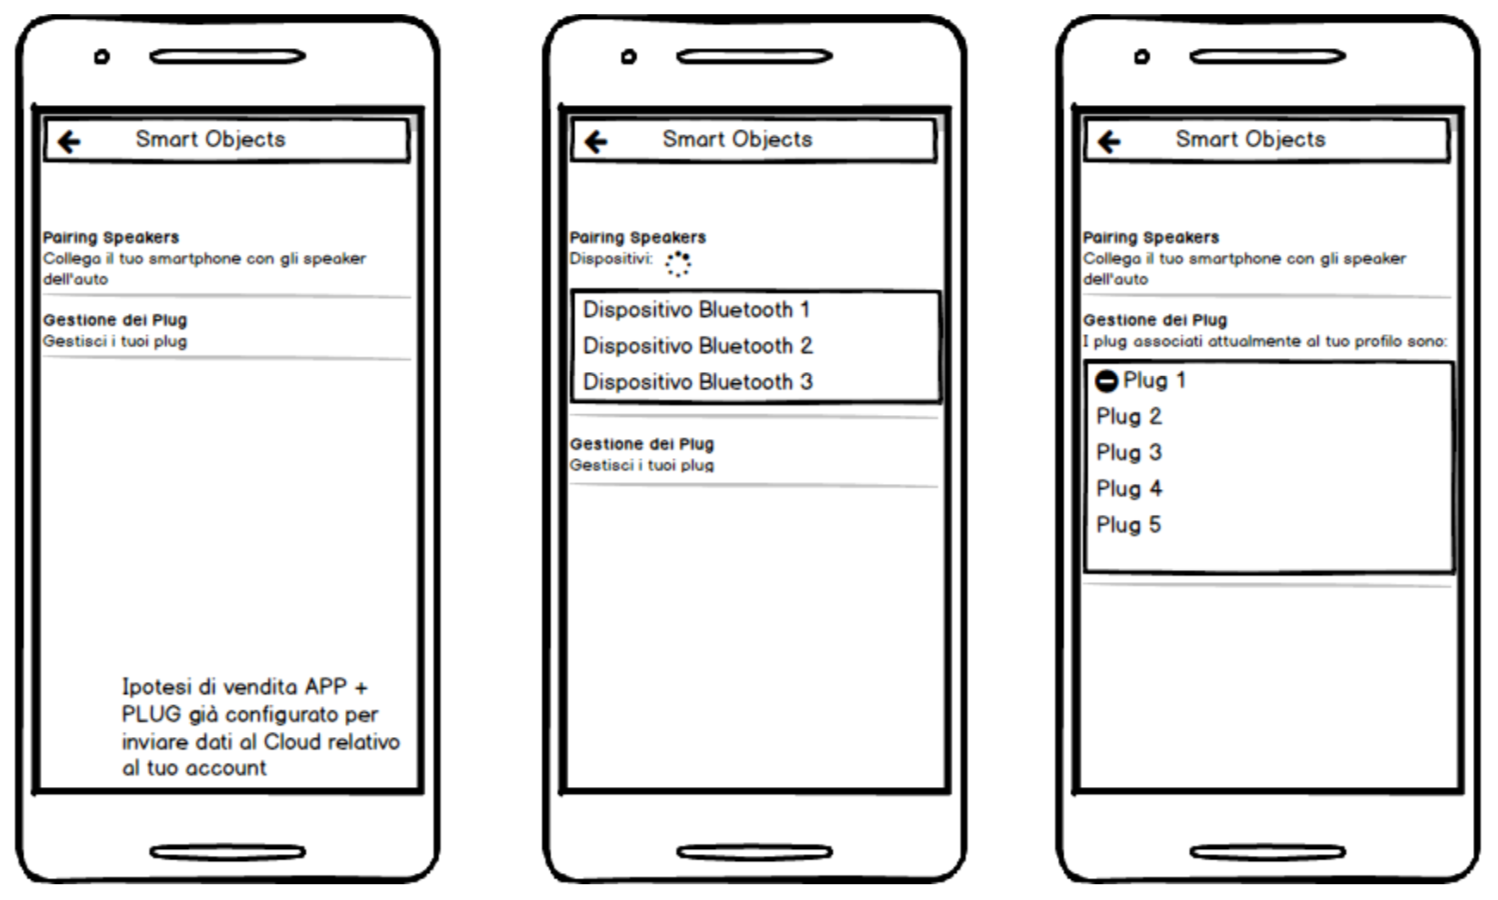
\includegraphics[width=\textwidth]{cpt/img/SmartObjectsPage.png}
\caption{Smart Objects Pages}
\end{figure}
\clearpage

\chapter{Future developments} \label{chap5}
The application can be improved by integrating the use of a \textit{text2speech} service that should have the role of reading the hints and send the relative audio to a speaker. This way the user will have the possibility to know about the hints during the drive.
\clearpage

\end{document}
